\cotefile{66}
\scanpage{2}
\noindent\begin{minipage}[t]{.10\linewidth}
\figure{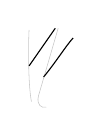
\begin{tikzpicture}[x=.28cm,y=.28cm]
\draw[gray!45,very thin] (.14,3.5) .. controls (.09,2.5) and (.12,.85) .. (.25,.25);
\draw (.14,1.87) -- (1.33,3.58);
\draw[gray!45,very thin] (1.46,3.58) -- (.57,.52) .. controls (.46,.1) and (.71,-.06) .. (.92,0);
\draw (.80,1.37) .. controls (1.34,2.02) and (1.81,2.78) .. (2.14,3.14);
\end{tikzpicture}}
\end{minipage}\hspace{.02\linewidth}%
\begin{minipage}[t]{.86\linewidth}
\tikz[baseline=(yr.base)]{\node[inner sep=2pt] (yr) {1964}; \draw (yr.north west) -- (yr.south west) -- (yr.south east) -- (yr.north east);}
\hfill Numéros cerclés sont sans doute difficiles.

\uline{Travaux de thèses}

\deleted{[\unsure{Collection} \unsure{1964}]}
\end{minipage}%
\begingroup\setlength{\marginparwidth}{2.9cm}\margin{(N.B. Les sujets 1 à 10 et 20, 21, \inserted{26, 27, 28} sont de nature essentiellement cohomologique \unsure{$\zeta$|$\xi$|§|$g$}. 10, 19, 23, 24, 25 \unsure{relèvent|relévent} de la théorie des intersections ; 11, 12, 13 se \unsure{rattachent} à la th. de Néron. 14, 15, 22 th. du topos...; 17, 18 yoga de \unsure{représentabilité}, \unsure{de|des} foncteurs)}\endgroup

1) Topologie et cohomologies $\mathrm{fppf}$ : formalisme \unsure{général|general}
\inserted{\textcircled{\scriptsize $*$} [Rela\uline{tion avec \unsure{coh-mologie|coho-mologie|cohomologie} cristall}ine]}

\reversemarginpar
\textcircled{2}\margin{[subordonné à 1), 11)]} \rule[.45ex]{3.9em}{.45pt} : dualité (\uline{locale}, globale).

\textcircled{3}\margin{[subordonné à 2), donc à 1) et 11)]} Partie $p$-primaire dans formule de Ogg-\unsure{Chafarévitch|Chafovévitch}

\normalmarginpar
\textcircled{4} Formule de RR en cohomologie étale, coeff. discrets.
\unsure{Relation|Relations} avec \unsure{représentation|représentations} d'Artin supérieures.
\inserted{[Formule du $\unsure{\chi|x}$ pour revêtement étale d'un schéma propre...]\unsure{.}}

5) Formule du $\chi$ pour V.A. avec anneau d'opérateurs (variante de Ogg-\unsure{chafarévitch}).

6) Formules de Lefschetz explicites (coeff. discrets étales, ou ``continus'' cohérents). Représentations d'Artin du point de vue cohérent....

\textcircled{7} Cohomologie des schémas de type fini sur $\mathbb{Z}$ ; théorèmes de dualité globale \unsure{satisfaisant|satisfaisants} (améliorant Artin).

\textcircled{8} \unsure{Formalisme|Formalismes} de dualité, du point de vue \inserted{complexes d'}opérateurs différentiels. Coefficients à connexion\unsure{..} intégrable .... \inserted{Lien avec ``cristaux''.}

\textcircled{9} Dualité analytique....

\tikz[baseline=(num.base)]{\node[draw,circle,inner sep=.7pt] (num) {\shortstack{10\\[-.5ex]\scriptsize$\unsure{\times|*}$}};}
Riemann-Roch et \unsure{pbs} connexes (faisceaux pseudo-cohérents de Modules), \inserted{\unsure{analytique|analytiques} ou algébrique.} \inserted{(\unsure{Cf|cf} SGA 6)}

\textcircled{\small 11} Structures et groupes de la catégorie des schémas morcelés. Foncteur de Néron relatif à un anneau de val. discrète.
% archive sheet number: 1

